\chapter[Analog Control]{Analog Control}
\label{ch:analog_control}
% This is copied out of:
% devBenGreen/latex/xiy_notes.tex

Using a quantum computer to simulate quantum dynamics requires the ability to generate Hamiltonians with programmable coefficients.
This requires us to develop a mapping between control voltages set by the experimentalist and the resultant Hamiltonian parameters.
We refer to this mapping as a control model.
We arrive at a control model with a two step calibration process described in this appendix.
In the first stage of the control model calibration, we use a series of single and two qubit measurements to infer
the parameters of the circuit model describing the device.  The details of the effective circuit model for this tunably coupled device were first worked out in \cite{Neill2018}.
In the second stage of the control model calibration, we use the many-body Ramsey technique to benchmark the collective
dynamics of the circuit, with all qubits coupled and near resonance with one another.
Next, we numerically optimize the control model parameters using the difference between the benchmarking data and control model predictions as a cost function.
This is the calibration procedure that was used to make the many-body localization measurements of chapter 5.

\section{Spectroscopy \label{sec:spectroscopy}}

In the first stage of calibration we use conventional probe tone spectroscopy to measure
the $\ket{0} \rightarrow \ket{1}$ and $\ket{1} \rightarrow \ket{2}$ transition frequencies for each qubit.
These measurements are made with all other qubits biased far off resonance.

In order to make these measurements, we apply a bias voltage to the qubit's flux bias control
and apply a variable frequency probe tone to the qubit's microwave control.
Then we read out the qubit's $\ket{1}$ population.
We identify the qubit's transition frequency as the probe frequency that gives maximum population transfer to the excited state.
This procedure is repeated as a function of qubit bias.
We similarly measure the $\ket{1} \rightarrow \ket{2}$ transition frequency,
which captures the nonlinearity of the device and ultimately controls the "Hubbard U" interaction term of our Bose-Hubbard Hamiltonian.
The resulting curves are fit parametrically to give circuit element values for our physical device model.
This is shown in Fig.~\ref{spectroscopy data}(a).

It is important to note that the effective inductance qubit is sensitive to the inductance of the coupler.
This enables us to infer the circuit parameters of the coupler by measuring the qubit frequency as a function of coupler bias.
Example data from this procedure is shown in Fig.~\ref{spectroscopy data}(b).

The direct qubit - qubit interaction strength cannot be characterized from single qubit measurements alone.
In order to measure the direct interaction, we use a two qubit swapping experiment as shown in Fig.~\ref{spectroscopy data}(c).
The hopping strength is inferred from the on resonance hopping rate.

\quickwidefig{0.95\columnwidth}{./PDF/circuit_modelling_thesis.pdf}
{
a) Qubit spectroscopy measurement circuit diagram, pulse sequence, and example data.
The error plot in the example data corresponds to the difference between the data points and prediction from the parameterized control model.
b) Coupler spectroscopy measurement circuit diagram, pulse sequence and example data.
c) Direct interaction "Chevron" measurement.  The Hamiltonian hopping coefficient is obtained from the on resonance hopping rate.
}
{spectroscopy data}

In the tables below we report our measured circuit model parameters.
We find circuit model parameters in good agreement with previous characterizations of this device.\cite{Neill2018}
\begin{table}
    \caption{Measured qubit parameters}
    \centering
    \begin{tabular}{ c c c c c c c}
        \hline \hline
        Qubit & $C$\,(fF) & $Lj_{0}$\,(nH)& $Lg_{total}$\,(nH)& $V_{offset}$\,(A.U.)& $V/ \Phi_{0}$\,(A.U.) & $g_{\text{readout}}$\,(MHz) \\
        \hline
        $q_1$ & 87.0 & 6.28 & 1.00 & 0.037 & 0.756 & 95.5 \\
        $q_2$ & 84.2 & 6.20 & 1.07 & 0.076 & 0.762 & 90.6  \\
        $q_3$ & 84.4 & 6.27 & 1.02 & 0.073 & 0.764 & 92.1  \\
        $q_4$ & 82.8 & 6.52 & 1.11 & 0.057 & 0.762 & 76.0  \\
        $q_5$ & 85.0 & 6.14 & 0.97 & 0.095 & 0.763 & 93.3  \\
        $q_6$ & 88.3 & 6.13 & 0.82 & 0.057 & 0.760 & 105.1 \\
        $q_7$ & 80.7 & 6.58 & 1.25 & 0.054 & 0.747 & 76.4  \\
        $q_8$ & 85.4 & 6.27 & 0.96 & 0.064 & 0.762 & 99.2  \\
        $q_9$ & 85.6 & 6.38 & 0.95 & 0.044 & 0.785 & 97.0  \\
        \hline
    \end{tabular}
    \label{table:Qubit Parameters}
\end{table}

\begin{table}
    \caption{Measured coupler parameters}
    \centering
    \begin{tabular}{ c c c c c c c c}
        \hline \hline
        Coupler & $M_{left}$\,(pH) & $M_{right}$\,(pH) & $\beta_{max}$ & $f_{0}$\,(GHz) & $V_{offset}$\,(A.U.) & $V / \Phi_{0}$\,(A.U.) \\ % & fudge \\
        \hline
$c_{1,2}$ & 45.0 & 42.3 & 0.675 & 15.1 & 0.694 & 0.965\\ % & 479115.3163698823 \\
$c_{2,3}$ & 45.4 & 41.6 & 0.678 & 14.9 & 0.683 & 0.964\\ % & 798459.7494982895 \\
$c_{3,4}$ & 45.1 & 42.8 & 0.684 & 15.0 & 0.682 & 0.956\\ % & 430696.97482430335 \\
$c_{4,5}$ & 46.1 & 41.3 & 0.681 & 14.9 & 0.685 & 0.961\\ % & -189375.77474641177\\
$c_{5,6}$ & 42.9 & 37.5 & 0.669 & 14.4 & 0.682 & 0.963\\ % & -495103.36686547904 \\
$c_{6,7}$ & 41.2 & 42.0 & 0.676 & 14.5 & 0.672 & 0.952\\ % & -832508.8345176188 \\
$c_{7,8}$ & 47.0 & 40.9 & 0.691 & 14.9 & 0.676 & 0.963\\ % & -502200.6315507185 \\
$c_{8,9}$ & 44.6 & 38.6 & 0.680 & 15.0 & 0.686 & 0.958\\ % & 1958451.7900973207 \\
        \hline
    \end{tabular}
    \label{table:Coupler Parameters}
\end{table}


%\begin{table}
%    \caption{Measured qubit parameters}
%    \centering
%    \begin{tabular}{ c c c c c c c}
%        \hline \hline
%        Qubit & C & $Lj_{0}$ & $Lg_{total}$ & $V_{offset}$ & $V/ \Phi_{0}$ & $\text{readout}_{g}$ \\
%        \hline
%        $q_1$ & 8.70-14 & 6.28-09 & 9.95-10 & 0.037 & 0.756 & 95496194  \\
%        $q_2$ & 8.42-14 & 6.20-09 & 1.07-09 & 0.076 & 0.762 & 90614175  \\
%        $q_3$ & 8.44-14 & 6.27-09 & 1.02-09 & 0.073 & 0.764 & 92096391  \\
%        $q_4$ & 8.28-14 & 6.52-09 & 1.11-09 & 0.057 & 0.762 & 76041127  \\
%        $q_5$ & 8.50-14 & 6.14-09 & 9.68-10 & 0.095 & 0.763 & 93350116  \\
%        $q_6$ & 8.83-14 & 6.13-09 & 8.22-10 & 0.057 & 0.760 & 105148979 \\
%        $q_7$ & 8.07-14 & 6.58-09 & 1.25-09 & 0.054 & 0.747 & 76450012  \\
%        $q_8$ & 8.54-14 & 6.27-09 & 9.58-10 & 0.064 & 0.762 & 99173392  \\
%        $q_9$ & 8.56-14 & 6.38-09 & 9.54-10 & 0.044 & 0.785 & 97020320  \\
%        \hline
%    \end{tabular}
%    \label{table:Qubit Parameters}
%\end{table}
%
%\begin{table}
%    \caption{Measured coupler parameters}
%    \centering
%    \begin{tabular}{ c c c c c c c c}
%        \hline \hline
%        Coupler & $M_{left}$ & $M_{right}$ & $\beta_{max}$ & $f_{0}$ & $V_{offset}$ & $V / \Phi_{0}$ \\ % & fudge \\
%        \hline
%        $c_{1,2}$ & 4.50-11 & 4.23-11 & 0.675 & 15.1 & 0.694 & 0.965\\ % & 479115.3163698823 \\
%        $c_{2,3}$ & 4.54-11 & 4.16-11  & 0.678 & 14.9 & 0.683 & 0.964\\ % & 798459.7494982895 \\
%        $c_{3,4}$ & 4.51-11  & 4.28-11 & 0.684 & 15.0 & 0.682 & 0.956\\ % & 430696.97482430335 \\
%        $c_{4,5}$ & 4.61-11  & 4.13-11  & 0.681 & 14.9 & 0.685 & 0.961\\ % & -189375.77474641177\\
%        $c_{5,6}$ & 4.29-11  & 3.75-11 & 0.669 & 14.4 & 0.682 & 0.963\\ % & -495103.36686547904 \\
%        $c_{6,7}$ & 4.12-11 & 4.20-11 & 0.676 & 14.5 & 0.672 & 0.952\\ % & -832508.8345176188 \\
%        $c_{7,8}$ & 4.70-11 & 4.09-11 & 0.691 & 14.9 & 0.676 & 0.963\\ % & -502200.6315507185 \\
%        $c_{8,9}$ & 4.46-11 & 3.86-11 & 0.680 & 15.0 & 0.686 & 0.958\\ % & 1958451.7900973207 \\
%        \hline
%    \end{tabular}
%    \label{table:Coupler Parameters}
%\end{table}


\section{Many-body Ramsey spectroscopy}
\label{sec:mbr}

Many-body Ramsey spectroscopy is the primary benchmarking technique for our multi-qubit, time-independent Hamiltonians\,\cite{Roushan2018}.
This technique allows us to extract the eigenvalues of a time independent Hamiltonian.
We can then compare the extracted eigenvalues with those predicted from our control model to establish a measure of fidelity.
In this appendix we give a detailed discussion of many-body Ramsey spectroscopy and its use in validating and optimizing our control model.

For a wavefunction $\ket{\psi}$ evolving under a time independent Hamiltonian $H$ we can write down the time dependence of $\ket{\psi}$ by expanding it in the
energy eigenbasis.

\begin{equation}
    \ket{\psi (t)} =e^{-i H t} \ket{\psi_{0}} = \sum_{\alpha} C_{\alpha} e^{-i E_{\alpha} t} \ket{\phi_{\alpha}}
    \label{ti_schrodinger_eqn}
\end{equation}

\noindent The coefficients $C_{\alpha}$ are given by the overlap of the initial state with the eigenstates of $H$.

\begin{equation}
    C_{\alpha} = \braket{\phi_{\alpha}|\psi_{0}}
\end{equation}

\noindent Looking at Eq.\,~\ref{ti_schrodinger_eqn}, it is clear that if we could simply Fourier transform the wavefunction, the task ef extracting the eigenvalues of $H$ would be complete.
Unfortunately, $\ket{\psi}$ is not an observable and our ability to interogate $\ket{\psi}$ is limited to measuring the expectation values of Hermitian operators.
\draftcomment{is limited to sampling bitstrings which may be averaged to give the expectation values of certain Hermitian operators.}
Such an observable $\hat{O}$ can be expanded in the energy basis as

\begin{equation}
    \label{observable}
    \hat{O} = \sum_{\alpha,\alpha^{\prime}} O_{\alpha,\alpha^{\prime}} \ket{\phi_{\alpha^{\prime}}} \bra{\phi_{\alpha}}
\end{equation}

\noindent The time dependent expectation value of this operator is

\begin{equation*}
    \label{derive_energy_differences}
    \begin{aligned}
        O(t) \equiv \langle \hat{O}(t) \rangle =\braket{\psi(t)|\hat{O}|\psi(t)} = \\[2.0ex]
        \left( \sum_{\beta} C^{*}_{\beta} e^{i E_{\beta} t} \ket{\phi_{\beta}} \right)
        \left( \sum_{\alpha,\alpha^{\prime}} O_{\alpha,\alpha^{\prime}} \ket{\phi_{\alpha^{\prime}}} \bra{\phi_{\alpha}} \right)
        \left( \sum_{\beta^{\prime}} C_{\beta^{\prime}} e^{- i E_{\beta^{\prime}} t} \ket{\phi_{\beta^{\prime}}} \right) = \\[2.0ex]
        \sum_{\alpha, \alpha^{\prime}, \beta, \beta^{\prime} }
        \braket{\phi_{\beta^{\prime}}|\phi_{\alpha^{\prime}}}
        \braket{\phi_{\beta}|\phi_{\alpha}}
        C_{\beta^{\prime}}^{*} C_{\beta} O_{\alpha, \alpha^{\prime}} e^{i (E_{\beta^\prime} - E_{\beta}) t} = \\[2.0ex]
        \sum_{\alpha, \alpha^{\prime}} C^{*}_{\alpha^{\prime}} C_{\alpha} O_{\alpha, \alpha^{\prime}} e^{- i (E_{\alpha^{\prime}} - E_{\alpha}) t}
    \end{aligned}
\end{equation*}

\noindent The time dependence of $O(t)$ exposes our central challenge.
For a generic initial state and a generic $\hat{O}$ the time series $O(t)$ does not isolate the eigenvalues of $H$.
Instead, the Fourier transform of $O(t)$ reports all \textit{energy differences} in the spectrum.
In order to isolate the eigenvalues, we must engineer the initial state and measurement observables such that we keep only terms with $E_{\alpha^{\prime}}=0$.

From an engineering perspective,
the above equation is still somewhat opaque because it describes the time dependence of an observable only in terms of the eigenbasis of $H$.
Typically, however, we use the Fock basis for initialization and measurement.
Thus, although the Hamiltonian evolution of the multi-qubit system is most naturally described in terms of the the eigenstates of $H$,
the initial state and measurement observable that we wish to engineer are best described in terms of a product of single qubit states.
Schematically, we can diagram our algorithm as follows:

\begin{center}
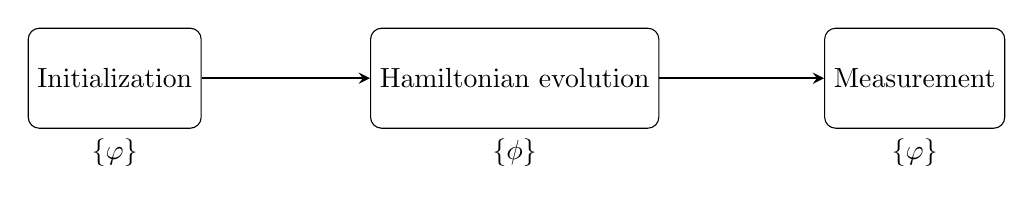
\begin{tikzpicture}[node distance=2in]
    \tikzstyle{process} = [rectangle, rounded corners, minimum width=0.5in, minimum height=0.5in,text centered, draw=black, fill=none]
    \tikzstyle{arrow} = [thick,->,>=stealth]
    \node (p1_label) [process, label=below:$\{\ket{\varphi}\}$] {Initialization};
    \node (p2_label) [process, right of=p1_label, xshift=0cm, label=below:$\{\ket{\phi}\}$] {Hamiltonian evolution};
    \node (p3_label) [process, right of=p2_label, xshift=0cm, label=below:$\{\ket{\varphi}\}$] {Measurement};
    \draw [arrow] (p1_label) -- (p2_label);
    \draw [arrow] (p2_label) -- (p3_label);
\end{tikzpicture}
\end{center}
where $\varphi$ and $\phi$ represent the Fock basis and Hamiltonian eigenbasis.

It is useful to work this out explicitly for the many-body Ramsey algorithm,
demonstrating the extraction of Hamiltonian eigenvalues
from the single photon manifold of a small three qubit system.  % in the zero and one photon manifolds.
%Consider the example of the vacuum + 1 photon subspace of a three qubit system.

The relevant Fock basis states are:
\begin{equation}
    \{\ket{\varphi\}} = \ket{000}, \ket{001}, \ket{010}, \ket{100}
\end{equation}
Initializing to a superposition state by doing a Y/2 rotation on a single qubit we have:
\begin{equation*}
    \ket{\psi_0} = \frac{1}{\sqrt{2}} \left( \ket{000} + \ket{001} \right) = \frac{1}{\sqrt{2}} \left( \ket{\varphi_0} + \ket{\varphi_1} \right)
\end{equation*}
Let C be the matrix that changes basis from the Fock basis to the eigenbasis of H.
\begin{equation}
    \ket{\psi_0}_{\phi} = \frac{1}{\sqrt{2}}
    \begin{bmatrix}
        1 & 0 & 0 & 0 \\
        0 & c_{11} & c_{12} & c_{13} \\
        0 & c_{21} & c_{22} & c_{23} \\
        0 & c_{31} & c_{32} & c_{33} \\
    \end{bmatrix}_{\varphi \rightarrow \phi}
    \begin{bmatrix}
        1 \\
        1 \\
        0 \\
        0 \\
    \end{bmatrix}_{\varphi}
    =
    \frac{1}{\sqrt{2}}
    \begin{bmatrix}
        1 \\
        c_{11} \\
        c_{21} \\
        c_{31} \\
    \end{bmatrix}_{\phi}
\end{equation}
Where the subscripts indicate which basis we are working in.
The time dependence of $\ket{\psi}$ is
\begin{equation}
    \ket{\psi(t)}_{\phi} =
    \begin{bmatrix}
        1 \\
        c_{11} e^{-i E_1 t} \\
        c_{21} e^{-i E_2 t} \\
        c_{31} e^{-i E_3 t}\\
    \end{bmatrix}_{\phi}
\end{equation}

We can apply the inverse transformation $C^{-1}$ to recover the time dependence of $\ket{\psi}$ in the Fock (measurement) basis.
\begin{equation*}
    \begin{aligned}
    \ket{\psi(t)}_{\varphi} & =
    C^{-1}\ket{\psi(t)}=
    \frac{1}{\sqrt{2}}
    \renewcommand*{\arraystretch}{1.5}
    \begin{bmatrix}
        1 & 0 & 0 & 0 \\
        0 & c^{-1}_{11} & c^{-1}_{12} & c^{-1}_{13} \\
        0 & c^{-1}_{21} & c^{-1}_{22} & c^{-1}_{23} \\
        0 & c^{-1}_{31} & c^{-1}_{32} & c^{-1}_{33} \\
    \end{bmatrix}_{\phi \rightarrow \varphi}
    \begin{bmatrix}
        1 \\
        c_{11} e^{-i E_1 t} \\
        c_{21} e^{-i E_2 t} \\
        c_{31} e^{-i E_3 t}\\
    \end{bmatrix}_{\phi}
    \\ & =
    \frac{1}{\sqrt{2}}
    \begin{bmatrix}
        1 \\
        c^{-1}_{11} c_{11} e^{-i E_1 t} +  c^{-1}_{12} c_{21} e^{-i E_2 t} + c^{-1}_{13} c_{31} e^{-i E_3 t} \\
        c^{-1}_{21} c_{11} e^{-i E_1 t} +  c^{-1}_{22} c_{21} e^{-i E_2 t} + c^{-1}_{23} c_{31} e^{-i E_3 t} \\
        c^{-1}_{31} c_{11} e^{-i E_1 t} +  c^{-1}_{32} c_{21} e^{-i E_2 t} + c^{-1}_{33} c_{31} e^{-i E_3 t} \\
    \end{bmatrix}_{\varphi}
    \equiv
    \frac{1}{\sqrt{2}}
    \begin{bmatrix}
    1 \\
    \varphi_{001}\\
    \varphi_{010}\\
    \varphi_{100}
    \end{bmatrix}
\end{aligned}
\end{equation*}

If we measure $\langle \sigma^x + i \sigma^y \rangle$ on site 1, then we have
\begin{equation}
\begin{bmatrix}
1 & \varphi_{001}^* & \varphi_{010}^* & \varphi_{100}^*
\end{bmatrix}
\begin{bmatrix}
0 & 1 & 0 & 0 \\
0 & 0 & 0 & 0 \\
0 & 0 & 0 & 0 \\
0 & 0 & 0 & 0 \\
\end{bmatrix}
\begin{bmatrix}
1 \\
\varphi_{001} \\
0 \\
0 \\
\end{bmatrix}
=
\begin{bmatrix}
1 & \varphi_{001}^* & \varphi_{010}^* & \varphi_{100}^*
\end{bmatrix}
\begin{bmatrix}
\varphi_{001} \\
0 \\
0 \\
0 \\
\end{bmatrix}
= \varphi_{001}
\end{equation}
In this case we recover the eigenvalues of H because \qeqn{ FFT(...) = a_1 \delta(E_1) + a_2 \delta(E_2) + a_3 \delta(E_3) }
where the $a_i$ are the coefficients coming from change of basis and normalization of the FFT.

This calculation makes the roles of the initial state and measurement observable clear.
It is essential that the initial state be a superposition of a reference state, and a state in the manifold that we wish to extract the eigenvalues of.
It is critical that the reference state is member of a manifold with trivial internal dynamics, in this case $\ket{\psi}_{ref} = \ket{000}$.
This state serves as an interference partner for our generalized Ramsey experiment,
and its triviality assures that the spectrum of our interference pattern is exclusively due to the dynamics of the target manifold and not the internal dynamics of the reference manifold.

The choice of $\hat{O} = \hat{a} = \hat{\sigma}^x + i \hat{\sigma}^y$ is also clarified by this calculation.
This operator interfers the dynamic manifold with the reference state, isolating the eigenvalues.

If we had instead chosen  $\hat{O} = \hat{\sigma}^x$ we would observe both positive and negative eigenvalues since

\begin{equation}
    \begin{bmatrix}
        1 & \varphi_{001}^* & \varphi_{010}^* & \varphi_{100}^{*}
    \end{bmatrix}
    \begin{bmatrix}
        0 & 1 & 0 & 0 \\
        1 & 0 & 0 & 0 \\
        0 & 0 & 0 & 0 \\
        0 & 0 & 0 & 0 \\
    \end{bmatrix}
    \begin{bmatrix}
        1 \\
        \varphi_{001} \\
        \varphi_{010} \\
        \varphi_{100} \\
    \end{bmatrix}
    =
    \begin{bmatrix}
        1 & \varphi_{001}^* & \varphi_{010}^* & \varphi_{100}^*
    \end{bmatrix}
    \begin{bmatrix}
         \varphi_{001}\\
        1 \\
        0 \\
        0 \\
    \end{bmatrix}
    =  \varphi_{001} + \varphi_{001}^*
\end{equation}
This is intuitive because for a single qubit precessing on the equator of the Bloch sphere measuring $<\sigma^x>$ alone does not indicate which direction the Bloch vector is precessing!

The naive attempt of measuring the on-site population of qubit 1 $\hat{n}_1$ yields the eigenvalue differences since
\begin{equation}
    \begin{bmatrix}
        1 & \varphi_{001}^* & 0 & 0
    \end{bmatrix}
    \begin{bmatrix}
        0 & 0 & 0 & 0 \\
        0 & 1 & 0 & 0 \\
        0 & 0 & 0 & 0 \\
        0 & 0 & 0 & 0 \\
    \end{bmatrix}
    \begin{bmatrix}
        1 \\
        \varphi_{001} \\
        0 \\
        0 \\
    \end{bmatrix}
    = \mid \varphi_{001} \mid^{2}
\end{equation}
The numerics below illustrate these points:
\begin{figure}[h]
    \begin{center}
        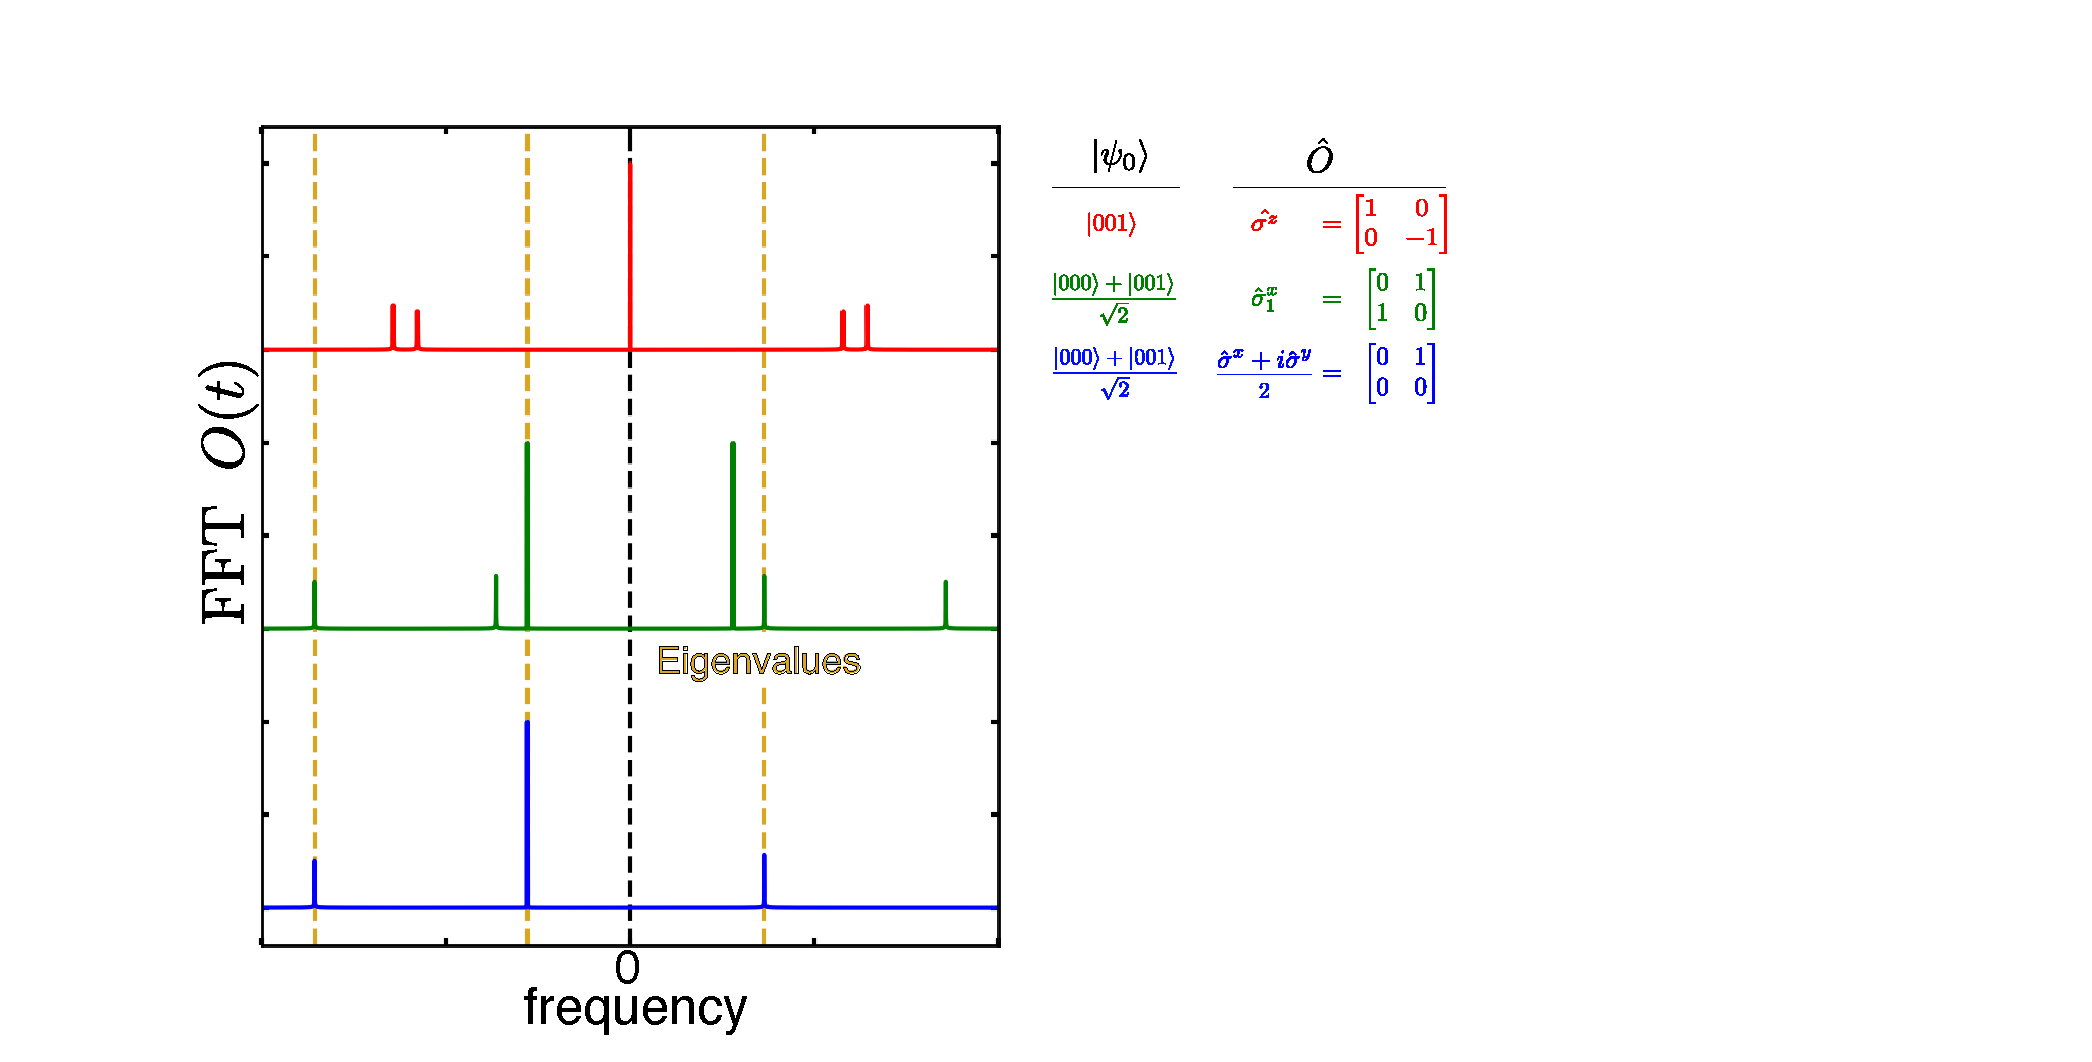
\includegraphics[width=250 mm]{./PDF/mbr_numerics_3qubit_o_psi0.pdf}
    \end{center}
    \caption{
    The spectrum of $\hat{O} = \sigma^z$ is comprised of the differences of eigenvalues.
    The spectrum of $\hat{O} = \sigma^x$ contains the eigenvalues and their mirrored frequencies.
    The spectrum of $\hat{O} = \sigma^x + i \sigma^y$ isolates the eigenvalues.
    }
    \label{mbr_peaks_numerics}
\end{figure}

\section{Control model optimization}

\begin{figure}[h]
    \begin{center}
        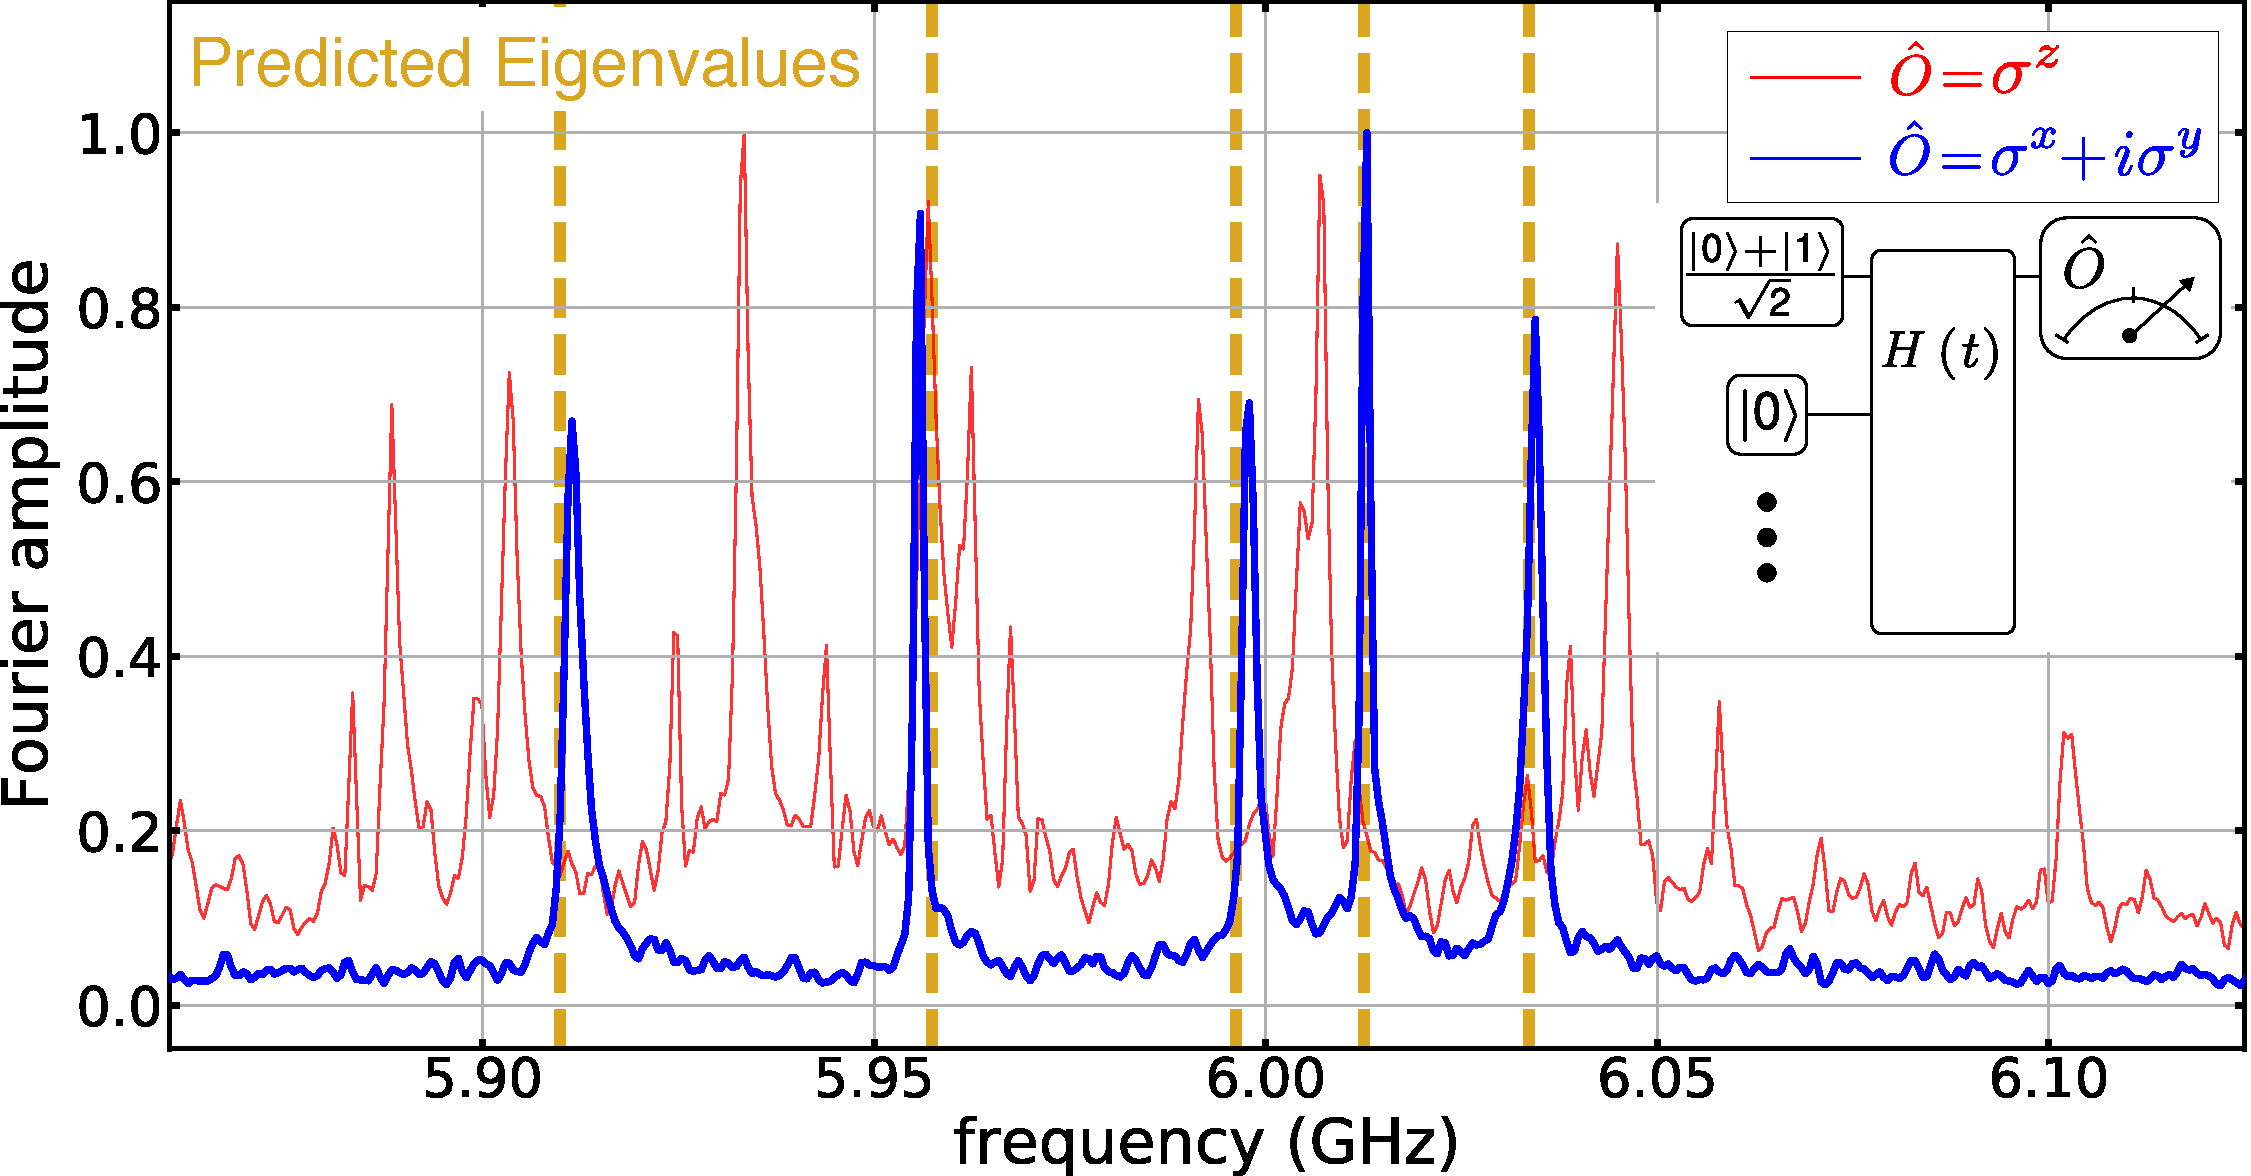
\includegraphics[width=150 mm]{./PDF/mbr_peaks_5q_data_191016_1057a.pdf}
    \end{center}
    \caption{\textbf{Many-body Ramsey five qubit data.}
    The fourier domain data for measurement observables
    $\langle \hat{O} \rangle =\langle \sigma^z \rangle$ (red) and $\langle \sigma^x + i \sigma^y \rangle$ (blue).
    The spectrum of $\left< \sigma^z (t) \right>$ is composed of artifacts from eigenvalue differences.
    The spectrum of $\left< \sigma^x (t) \right> + i \left< \sigma^y (t) \right>$ recovers the eigenvalues of $H$.
    }
    \label{mbr_peaks_data}
\end{figure}
Because the Many-body Ramsey extracts the eigenvalues of the Hamiltonian that was actually generated in the experiment,
we can compare the extracted eignevalues with those predicted by our circuit parameterization and use the difference as a control error metric.
With this error metric established, we can optimize the parameters of our control model to give a more accurate parameterization of the circuit.

\begin{figure}[h]
    \begin{center}
        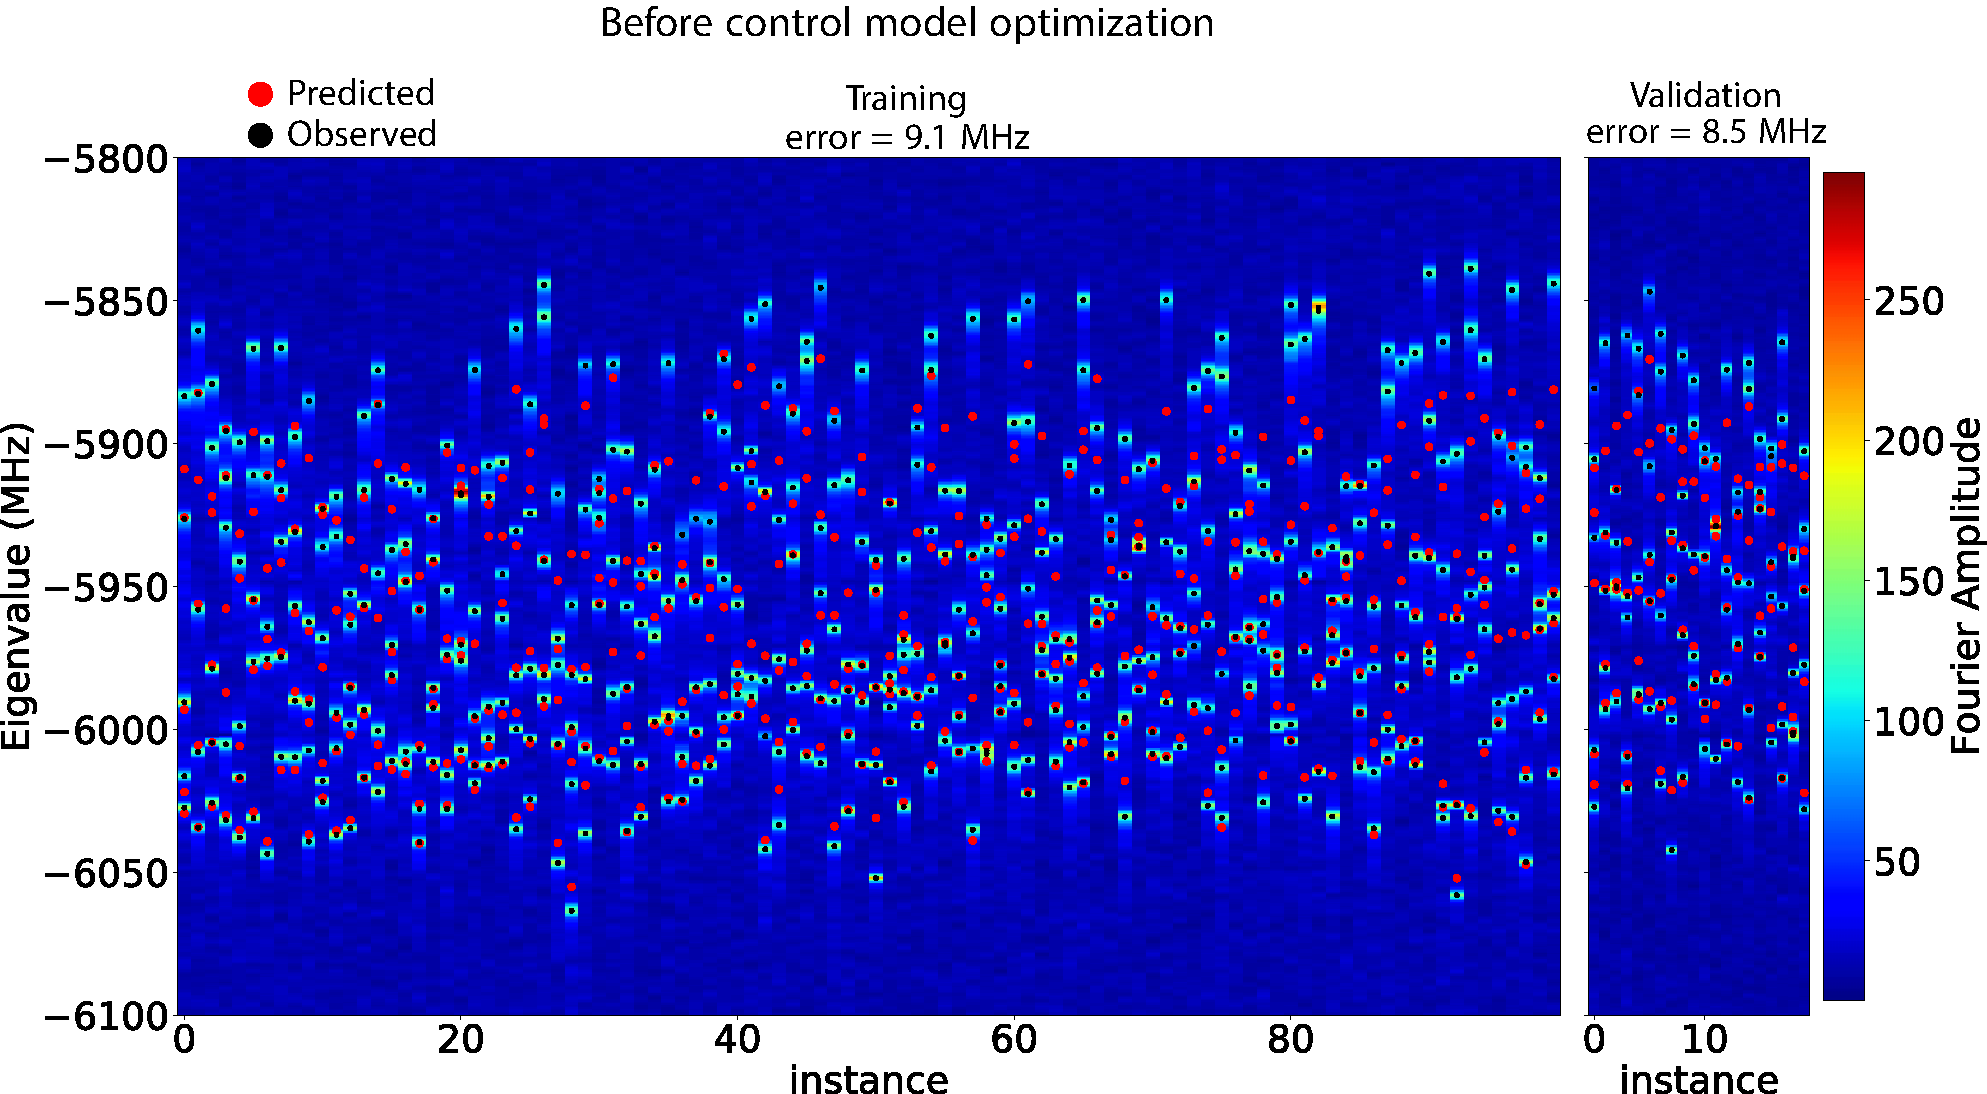
\includegraphics[width=150 mm]{./PDF/fourier_amp_2d_tv_pre_v2.pdf}
    \end{center}
        \caption{
        Five qubit many-body Ramsey spectroscopy data overlayed with predictions from control model prior to optimization.
        }
    \label{mbr_benchmark_pre_optimization}
\end{figure}
After using the conventional spectroscopy, described in above in section \ref{sec:spectroscopy}, to measure the circuit model parameters
using a series of single and two qubit measurements we benchmark the collective dynamics of the full system using the many-body Ramsey technique
described in section~\ref{sec:mbr}

The result is shown in fig.~\ref{mbr_benchmark_pre_optimization}.
The 2D color plot is the raw Fourier data for each of 100 training instances.
This data is overlayed with the control model predictions (red circles) and peak positions extracted with our analysis algorithm (black circles).
The error per eigenvalue is extracted to be $9$ MHz.
This is a large error, primarily resulting from the fact that the control bias conditions are different when we characterize
the single and two qubit systems and when we characterize the full system collective dynamics.

\begin{figure}[h]
    \begin{center}
        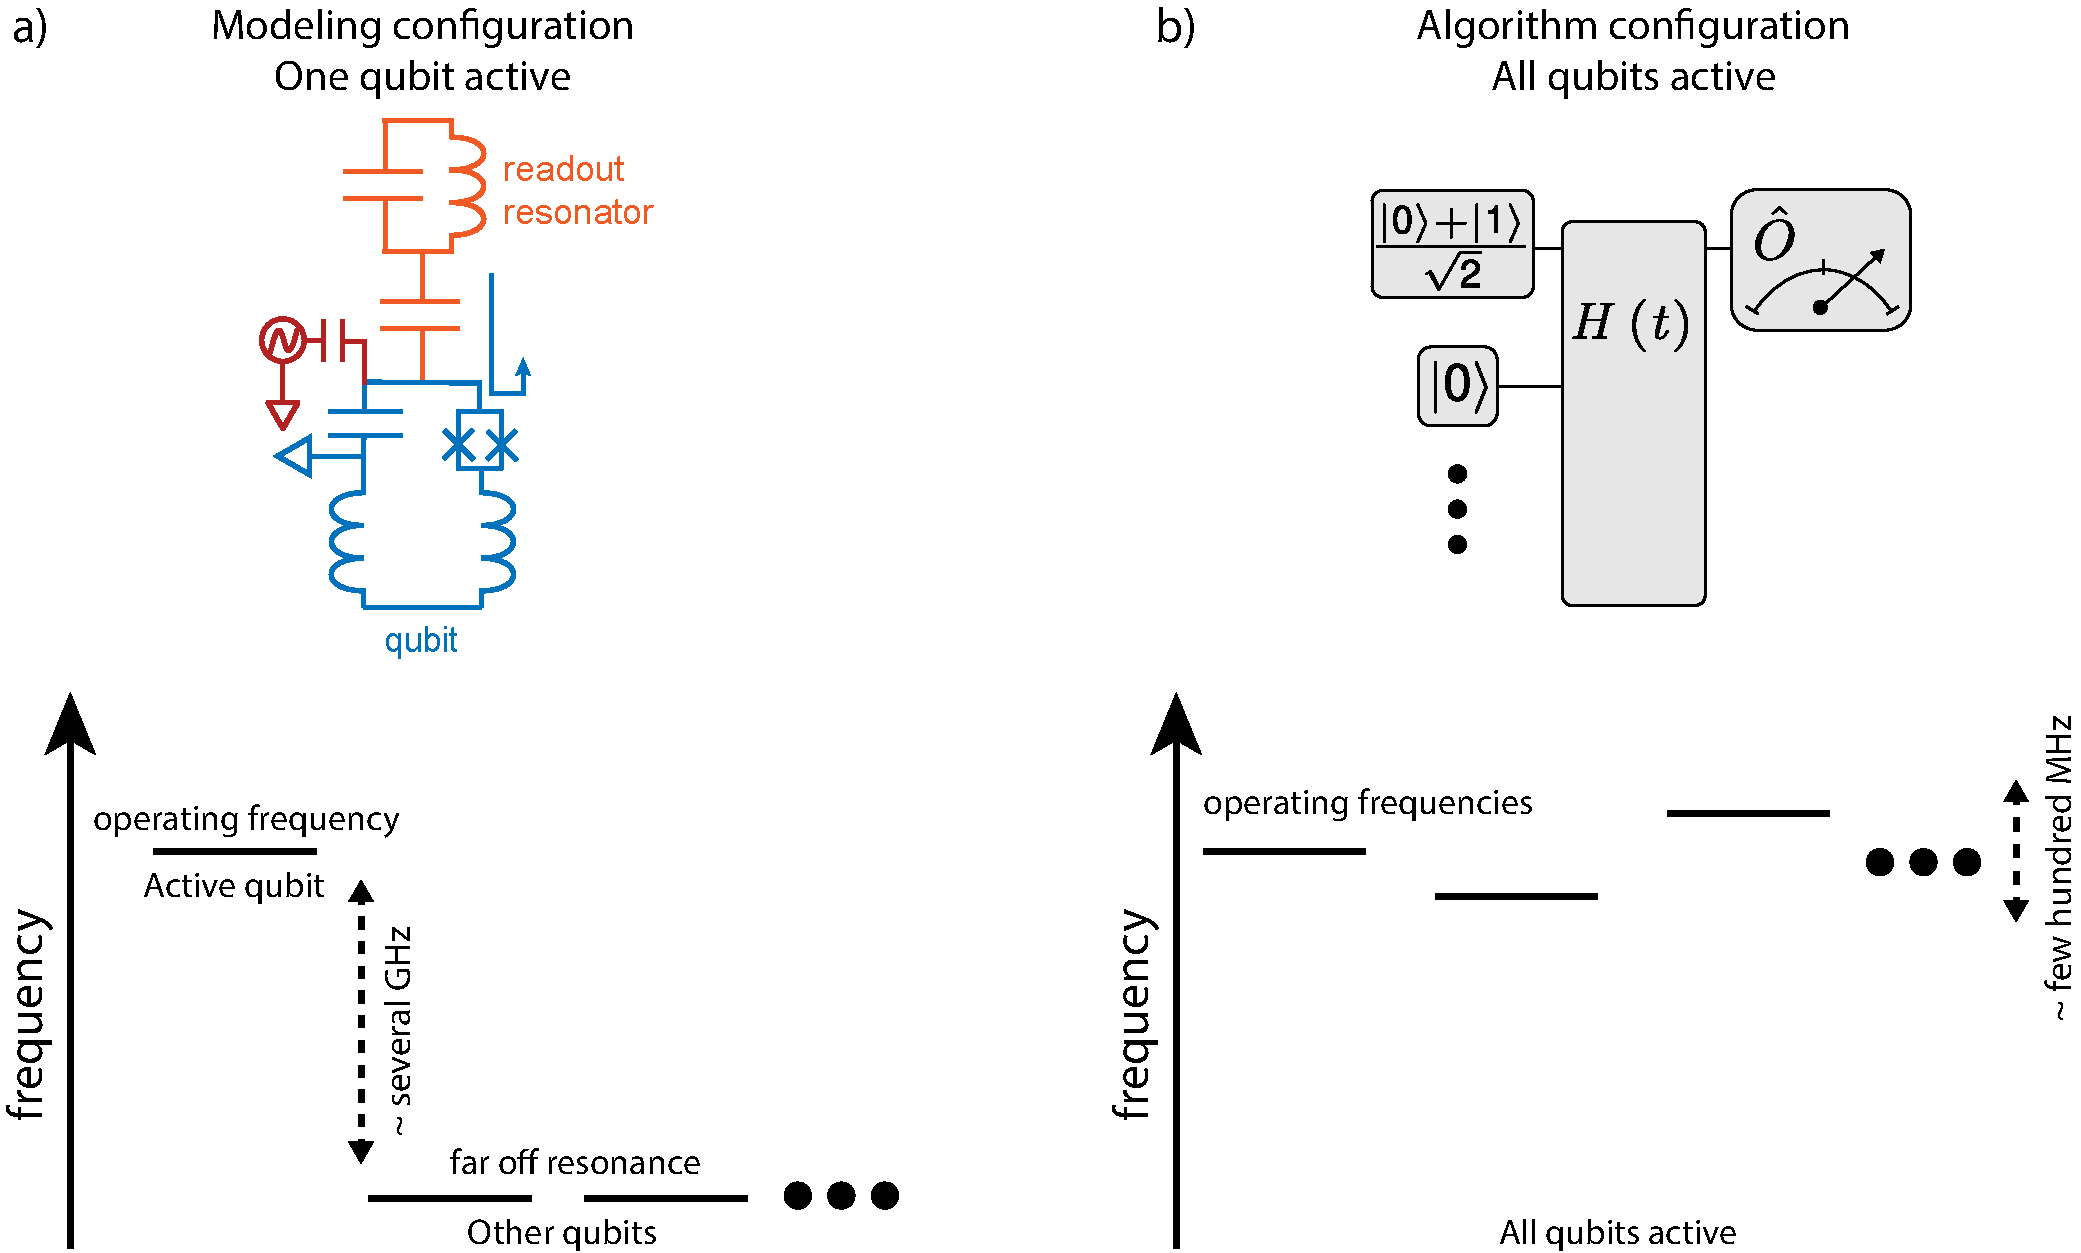
\includegraphics[width=150 mm]{./PDF/bias_configurations.pdf}
    \end{center}
    \caption{
    Schematic illustrating the qubit frequency configurations for the modelling spectroscopy experiments \textbf{(a)} and the Many-body Ramsey benchmarking experiments \textbf{(b)}.
    }
    \label{bias_configurations}
\end{figure}

\begin{figure}[h]
    \begin{center}
        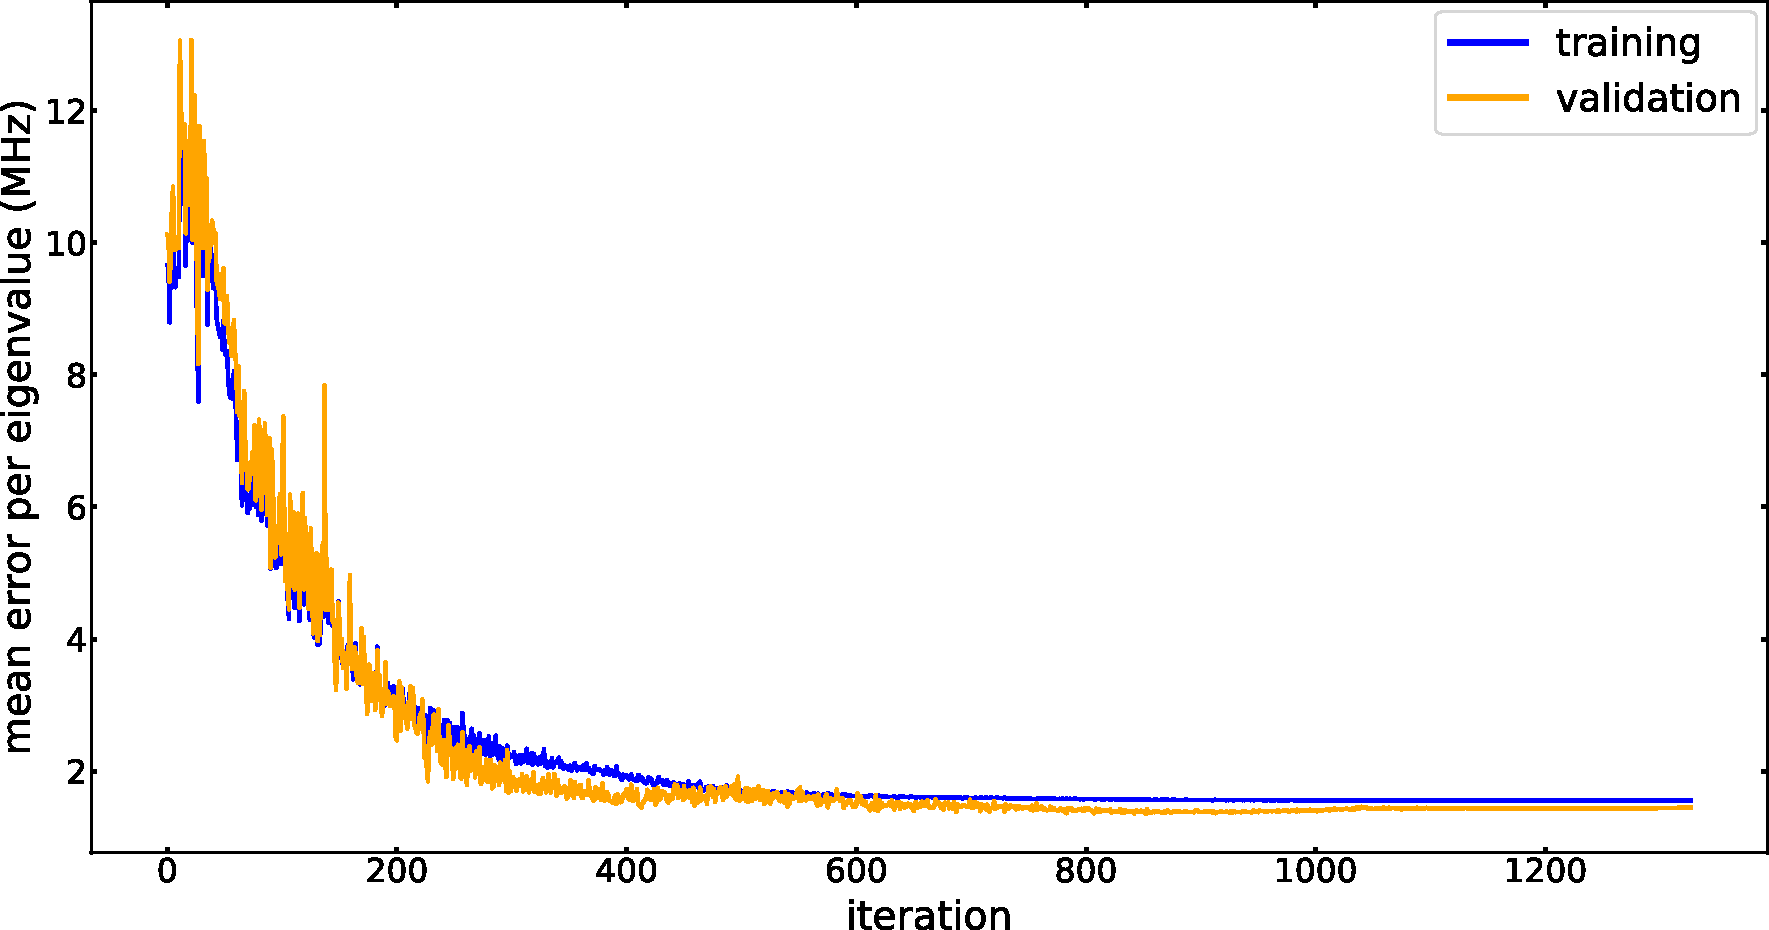
\includegraphics[width=150 mm]{./PDF/tv_error_during_opt.pdf}
    \end{center}
        \caption{
        Error per eigenvalue for the training and validation splits during optimization.
        Data shown is for five qubit Hamiltonians.
        }
    \label{error_during_optimization_training_validation}
\end{figure}
%The 5 qubit data in fig.~\ref{error_during_optimization_training_validation} illustrates this process.
Next, we follow the standard optimization procedure of dividing our full data set into training and validation subsets.
We then optimize the control model by minimizing the average error per eigenvalue of the training data only.
The error per eigenvalue at each iteration of the optimization process is shown in fig.~\ref{error_during_optimization_training_validation}.
\begin{figure}[h]
    \begin{center}
        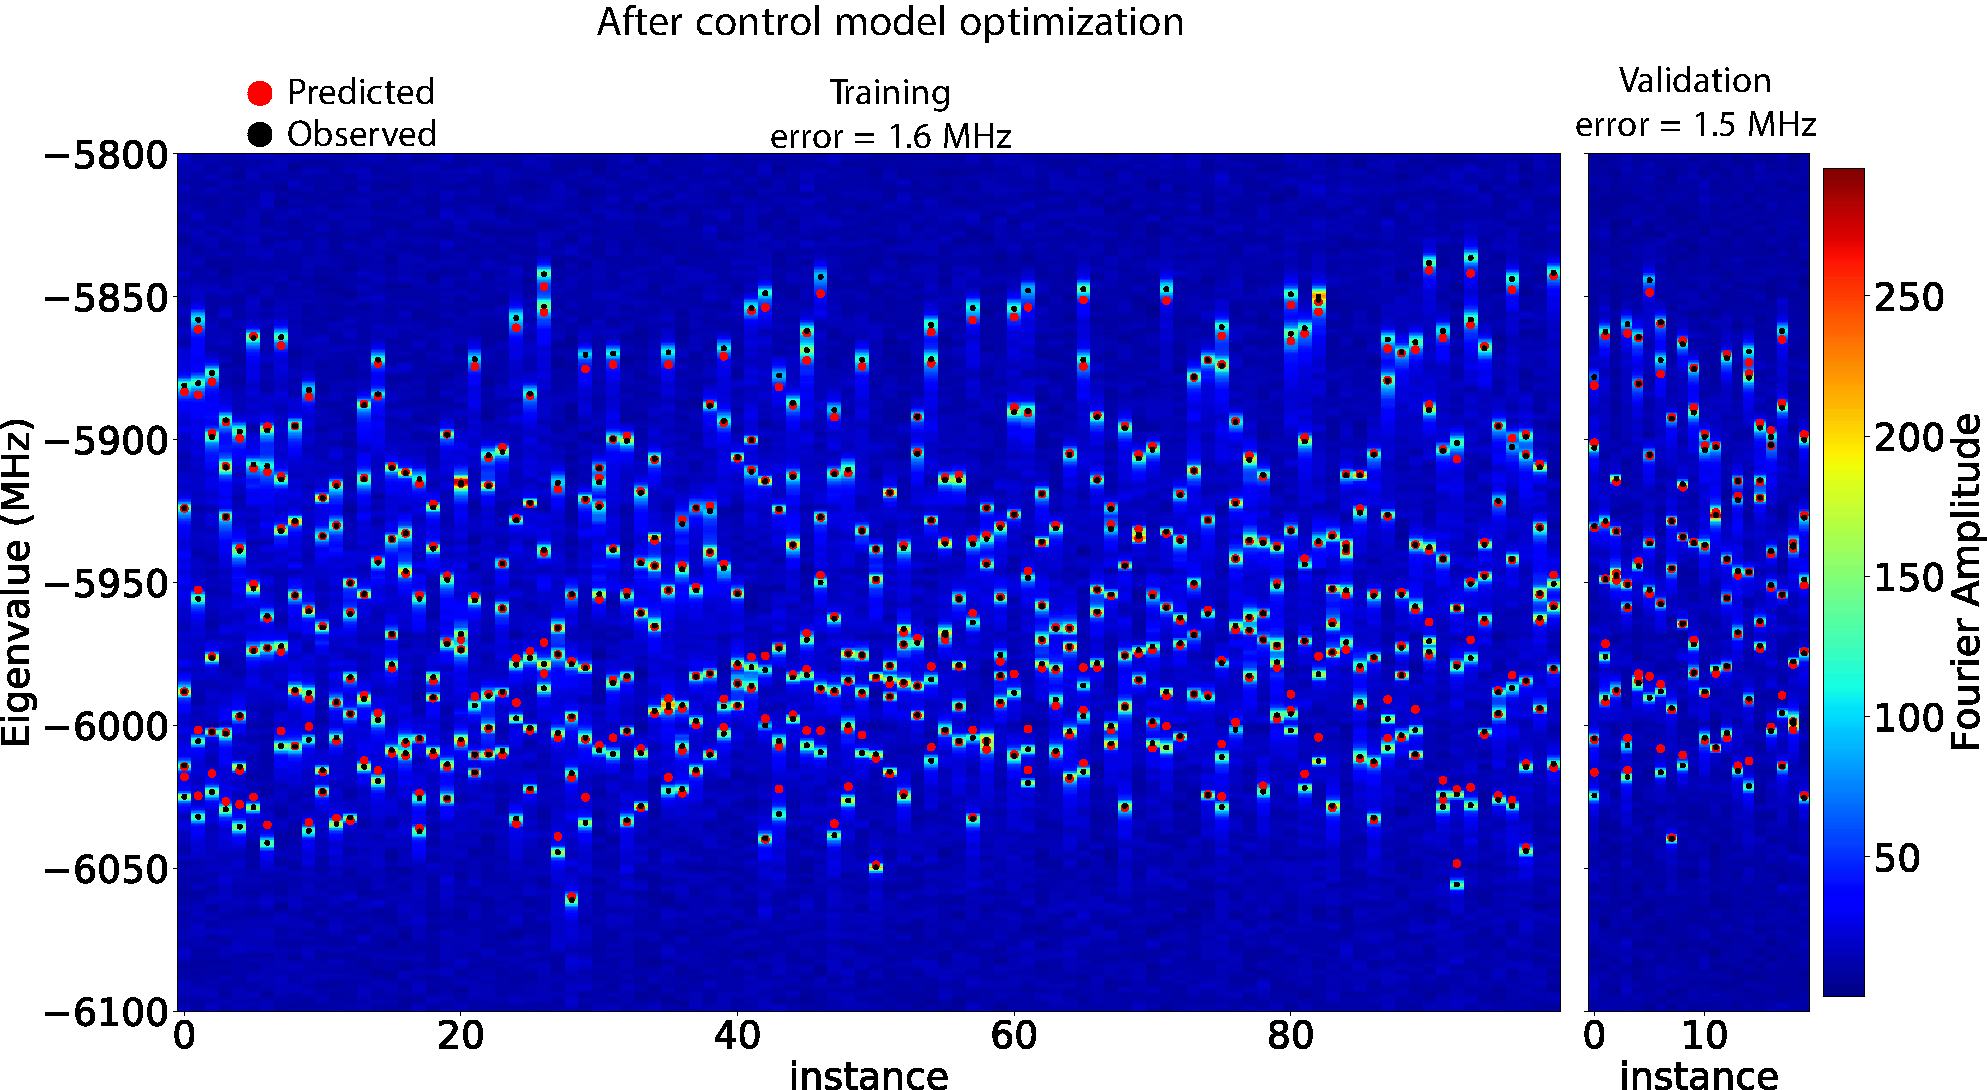
\includegraphics[width=150 mm]{./PDF/fourier_amp_2d_tv_post_v2.pdf}
    \end{center}
        \caption{
        Five qubit many-body Ramsey spectroscopy data overlayed with predictions from control model after optimization.
        }
    \label{mbr_benchmark_post_optimization}
\end{figure}
The predictions from the optimized control model are overlayed on the original fourier data in fig.~\ref{mbr_benchmark_post_optimization}

\begin{figure}[h]
    \begin{center}
        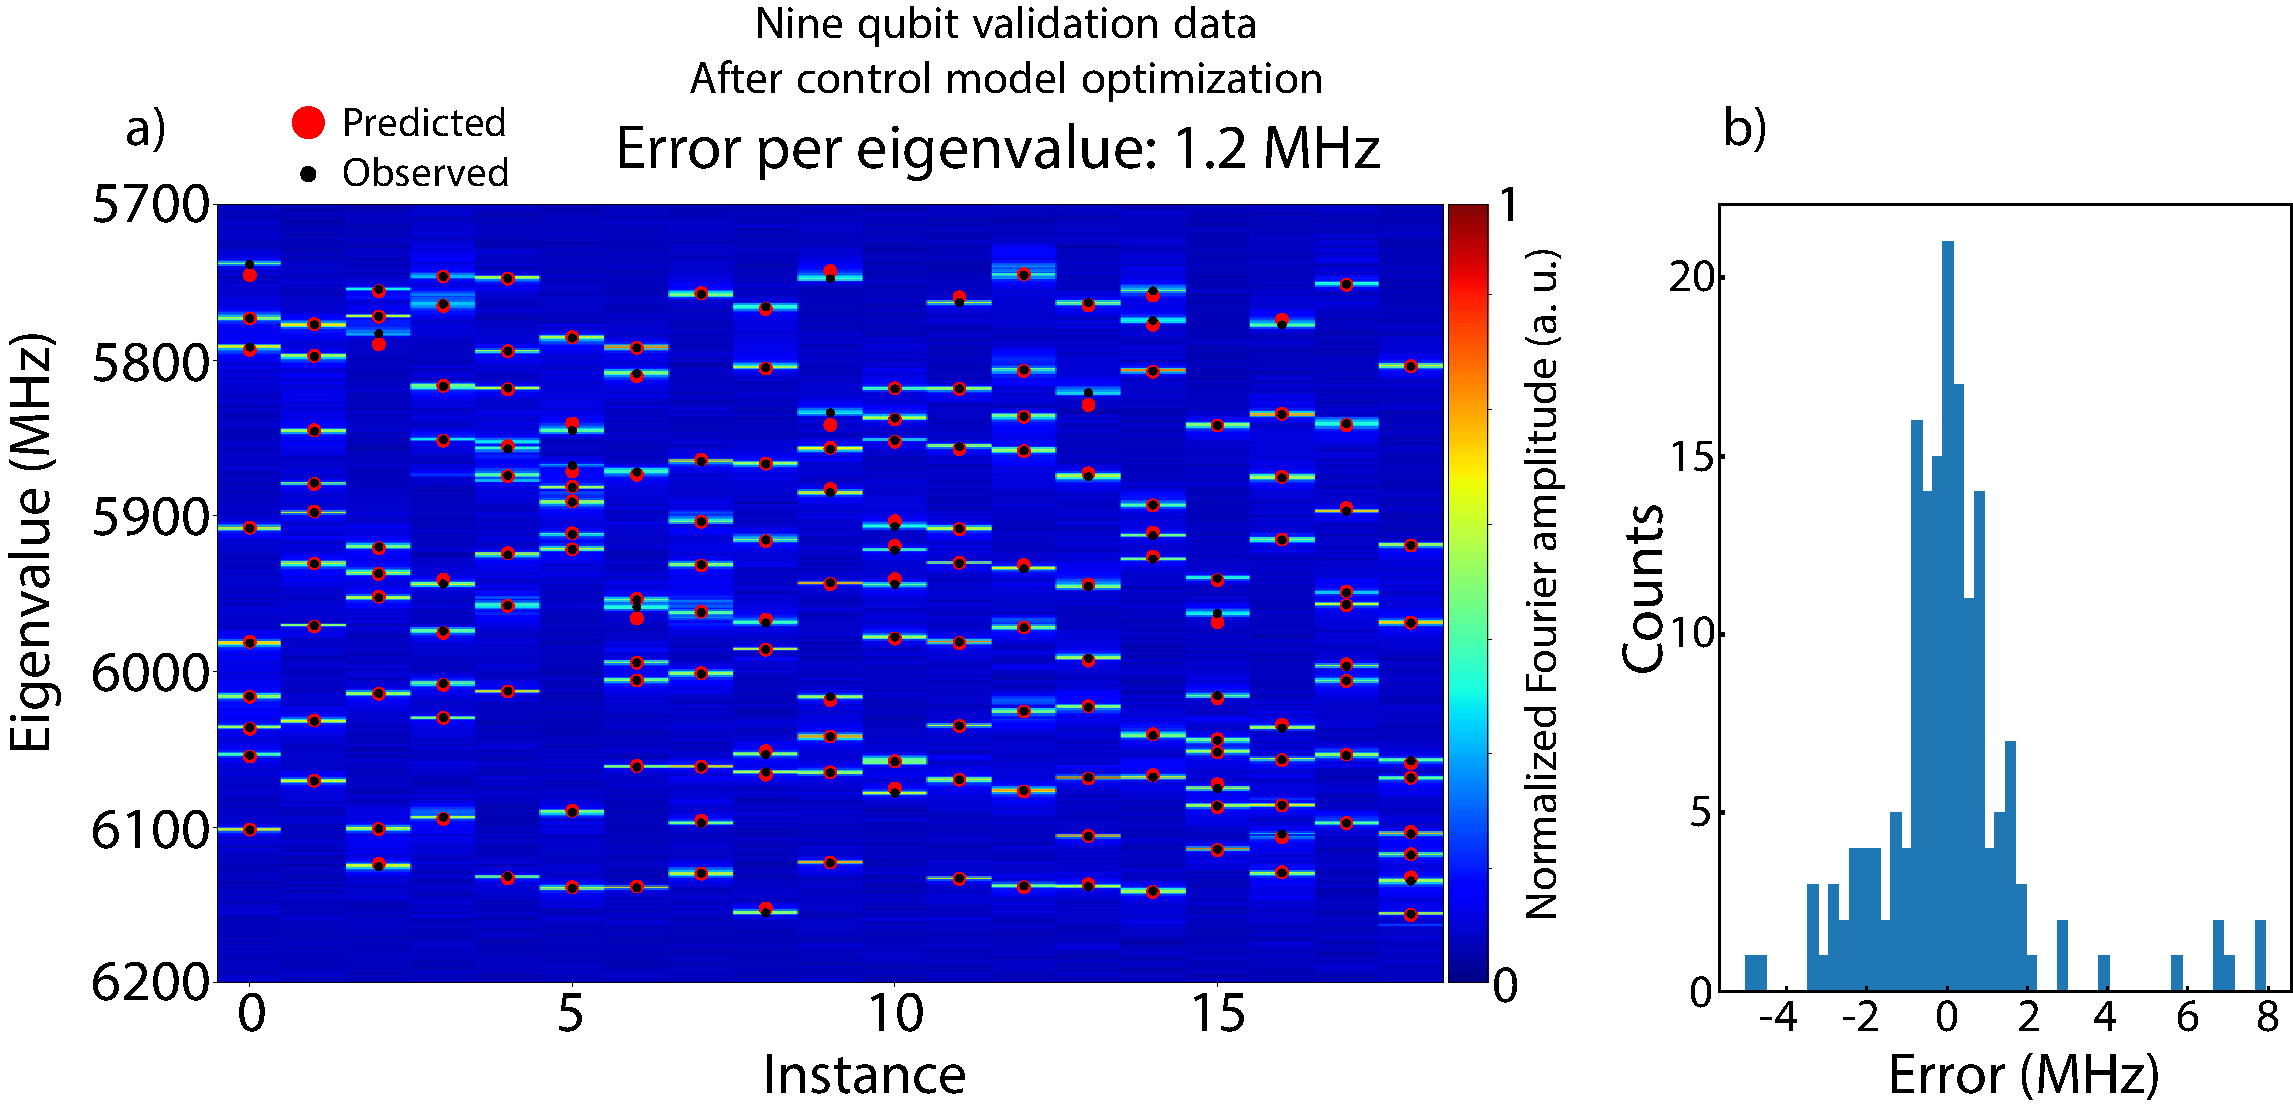
\includegraphics[width=150 mm]{./PDF/mbr_9q_validation.pdf}
    \end{center}
        \caption{\textbf{Manybody Ramsey calibration data for a nine qubit linear chain}
        a) Raw Fourier data from Many-body Ramsey spectroscopy.  b) Histogram of errors for each eigenvalue.
        }
    \label{9q manybody ramsey validation}
\end{figure}
In fig.~\ref{9q manybody ramsey validation} we show 9 qubit validation data with a validation error rate of 1.2 MHz per eigenvalue.
This shows that the MHz level error rate is maintained as we scale to larger numbers of qubits.

\draftcomment{
\section{Notes in progress}
Because the Bose-Hubbard Hamiltonian that we evolve the system under is photon conserving it takes the following form:
\begin{equation}
H=
\begin{bmatrix}
1 & 0 & 0 & 0 \\
0 & H_{11} & H_{12} & H_{13} \\
0 & H_{21} & H_{22} & H_{23} \\
0 & H_{31} & H_{32} & H_{33} \\
\end{bmatrix}
\end{equation}
Skipping over some algebra that is in my notebook.
Evolving under the H gives $\ket{\psi(t)}$
In the Energy basis
\begin{equation}
\ket{\psi (t)} = \frac{1}{\sqrt{2}}
\begin{bmatrix}
1 \\
a_{11} e^{-i E_1 t} + a_{12} e^{-i E_2 t} + a_{13} e^{-i E_3 t} \\
a_{21} e^{-i E_1 t} + a_{22} e^{-i E_2 t} + a_{23} e^{-i E_3 t} \\
a_{31} e^{-i E_1 t} + a_{32} e^{-i E_2 t} + a_{33} e^{-i E_3 t}
\end{bmatrix}
\end{equation}
Consider the case where the operator O is defined as X+iY on a single qubit
\begin{equation}
    O = \sigma^{x} + i \sigma^{y} =
    \begin{bmatrix}
        0 & 1 \\
        1 & 0
    \end{bmatrix}
    +
    i
    \begin{bmatrix}
        0 & -i \\
        i & 0
    \end{bmatrix}
    =
    \begin{bmatrix}
        0 & 1 \\
        0 & 0
    \end{bmatrix}
\end{equation}

In this case the only term that we keep is
\begin{equation}
    \ket{\phi_{\alpha}^{\prime}}
    \bra{\phi_{\alpha}}=
    \ket{0}
    \bra{1}
\end{equation}

so that

\begin{equation}
    \left< O \right>(t) = C^{*}_{0}C_{1} \: O_{1,0} \: e^{- i(E_{0} - E_{1} )t}
\end{equation}

There are a few comments here.

It is intuitive that we need to begin in a superposition state to form an interference pattern.
We can also see that this is the case from the algebra above:  If either $C_0$ or $C_1$ = 0 then $\left< O \right>(t)$=0

We also see that $\frac{ \ket{\text{vac}} + \ket{\text{target}} }{\sqrt{2}}$ Will give the strongest signal.
If other states are part of the superposition, they will reduce the visibility due to normalization, but they will not add more frequencies.

Let's be more explicit about how this works for a 3x3 example.
\begin{equation*}
    \begin{aligned}
        O(t) =\braket{\psi(t)|\hat{O}|\psi(t)} = \sum_{\alpha, \alpha^{\prime}} C^{*}_{\alpha^{\prime}} C_{\alpha} O_{\alpha, \alpha^{\prime}} e^{- i (E_{\alpha^{\prime}} - E_{\alpha}) t}   \\[2.0ex]
    \end{aligned}
\end{equation*}

In the energy basis $\ket{\phi}$:
\begin{equation*}
    \ket{\psi_0} = a\ket{\phi_1} + b\ket{\phi_2} + c\ket{\phi_3}
\end{equation*}
so that
\begin{equation*}
    \ket{\psi (t)} = a\ket{\phi_1}e^{-i E_1 t} + b\ket{\phi_2}e^{-i E_2 t} + c\ket{\phi_3}e^{-i E_3 t}
\end{equation*}
and with
\begin{equation*}
    O =
    \begin{bmatrix}
        O_{11} & O_{12} & O_{13}\\
        O_{21} & O_{22} & O_{23}\\
        O_{31} & O_{32} & O_{33}\\
    \end{bmatrix}
\end{equation*}
we have
\begin{equation*}
    \begin{aligned}
        \braket{\psi(t)|\hat{O}|\psi(t)} = \\[2.0ex]
        \begin{bmatrix}
            c_1^* e^{i E_1 t} & c_2^* e^{i E_2 t} & c_3^* e^{i E_3 t}
        \end{bmatrix}
        \begin{bmatrix}
            O_{11} & O_{12} & O_{13}\\
            O_{21} & O_{22} & O_{23}\\
            O_{31} & O_{32} & O_{33}\\
        \end{bmatrix}
        \begin{bmatrix}
            c_1 e^{-i E_1 t} \\
            c_2 e^{-i E_2 t} \\
            c_3 e^{-i E_3 t}
        \end{bmatrix} = \\[2.0 ex]
        c_1^* e^{i E_1 t} \left( c_1 O_{11} e^{-i E_1 t} + c_2 O_{12} e^{-i E_2 t} + c_3 O_{13} e^{-i E_3 t} \right) + \mathellipsis
    \end{aligned}
\end{equation*}
From the above equation it is clear that without a reference state we will get energy differences and not energy eigenvalues.
We can fix this problem and measure the eigenvalues by including a reference state that is decoupled from the dynamics of the 3x3 subspace and serves as an interference partner for a Ramsey measurement.
The natural choice is the vacuum state.
Taking the reference (vacuum) state to have zero energy and decoupled from the manifold that we wish to measure the eigenvalues of:
\begin{equation*}
    \ket{\psi (t)} = c_0\ket{\phi_{ref}} + c_1\ket{\phi_1}e^{-i E_1 t} + c_2\ket{\phi_2}e^{-i E_2 t} + c_3\ket{\phi_3}e^{-i E_3 t}
\end{equation*}
and
\begin{equation*}
O =
\begin{bmatrix}
O_{00} & O_{01} & O_{02} & O_{03}\\
O_{10} & O_{11} & O_{12} & O_{13}\\
O_{20} & O_{21} & O_{22} & O_{23}\\
O_{30} & O_{31} & O_{32} & O_{33}\\
\end{bmatrix}
\end{equation*}
which leads to

\begin{equation*}
    \begin{aligned}
        \braket{\psi(t)|\hat{O}|\psi(t)} = \\[2.0ex]
        \begin{bmatrix}
            c_0^* & c_1^* e^{i E_1 t} & c_2^* e^{i E_2 t} & c_3^* e^{i E_3 t}
        \end{bmatrix}
        \begin{bmatrix}
            O_{00} & O_{01} & O_{02} & O_{03}\\
            O_{10} & O_{11} & O_{12} & O_{13}\\
            O_{20} & O_{21} & O_{22} & O_{23}\\
            O_{30} & O_{31} & O_{32} & O_{33}\\
        \end{bmatrix}
        \begin{bmatrix}
            c_0  \\
            c_1 e^{-i E_1 t} \\
            c_2 e^{-i E_2 t} \\
            c_3 e^{-i E_3 t}
        \end{bmatrix} = \\[2.0 ex]
        c_0^* \left( c_0 O_{00} + c_1 O_{01} e^{-i E_1 t} + c_2 O_{02} e^{-i E_2 t} + c_3 O_{03} e^{-i E_3 t} \right)& + \\[2.0 ex]
        c_1^* e^{i E_1 t} \left( c_0 O_{10} + c_1 O_{11} e^{-i E_1 t} + c_2 O_{12} e^{-i E_2 t} + c_3 O_{13} e^{-i E_3 t} \right)& +\\[2.0 ex]
        c_2^* e^{i E_2 t} \left( c_0 O_{20} + c_1 O_{21} e^{-i E_1 t} + c_2 O_{22} e^{-i E_2 t} + c_3 O_{23} e^{-i E_3 t} \right)& +\\[2.0 ex]
        c_3^* e^{i E_3 t} \left( c_0 O_{30} + c_1 O_{31} e^{-i E_1 t} + c_2 O_{32} e^{-i E_2 t} + c_3 O_{33} e^{-i E_3 t} \right)& \\[2.0 ex]
    \end{aligned}
\end{equation*}


\subsection{simple example}
For analog control our measurement basis is different than the dynamic basis.
\begin{equation*}
    %\begin{aligned}
    \ket{\psi} \implies \textrm{the wavefunction}
    \ket{\varphi} \implies \textrm{The measurement / initialization / Fock basis}
    \ket{\phi} \implies \textrm{The measurement / Fock basis}
    %\end{aligned}
\end{equation*}

Consider the example of the vacuum + 1 photon subspace of a three qubit system:
the Fock basis states are:
\begin{equation*}
    \varphi = \ket{000}, \ket{001}, \ket{010}, \ket{100}
\end{equation*}
Initializing to a superposition state by doing a Y/2 pulse we have:
\begin{equation*}
    \psi = \frac{1}{\sqrt{2}} \left( \ket{000} + \ket{001} \right) = \frac{1}{\sqrt{2}} \left( \ket{\varphi_0} + \ket{\varphi_1} \right)
\end{equation*}

\begin{equation}
    H=
    \begin{bmatrix}
        1 & 0 & 0 & 0 \\
        0 & H_{11} & H_{12} & H_{13} \\
        0 & H_{21} & H_{22} & H_{23} \\
        0 & H_{31} & H_{32} & H_{33} \\
    \end{bmatrix}
\end{equation}

Skipping over some algebra that is in my notebook.

In the Energy basis
\begin{equation}
    \ket{\psi (t)} = \frac{1}{\sqrt{2}}
    \begin{bmatrix}
        1 \\
        a_{11} e^{-i E_1 t} + a_{12} e^{-i E_2 t} + a_{13} e^{-i E_3 t} \\
        a_{21} e^{-i E_1 t} + a_{22} e^{-i E_2 t} + a_{23} e^{-i E_3 t} \\
        a_{31} e^{-i E_1 t} + a_{32} e^{-i E_2 t} + a_{33} e^{-i E_3 t}
    \end{bmatrix}
\end{equation}

Now we can compare measurements with different operators on different initial states.
\begin{equation}
    \hat{a}_1 = \ket{000}\bra{001} =
    \begin{bmatrix}
        0 & 1 & 0 & 0 \\
        0 & 0 & 0 & 0 \\
        0 & 0 & 0 & 0 \\
        0 & 0 & 0 & 0 \\
    \end{bmatrix}
\end{equation}

\begin{equation}
    \braket{\psi(t)|\hat{a}_1|\psi(t)} = a_{11} e^{-i E_1 t} + a_{12} e^{-i E_2 t} + a_{13} e^{-i E_3 t}
\end{equation}

\begin{equation}
    \hat{n}_1 = \ket{001}\bra{001} =
    \begin{bmatrix}
        0 & 0 & 0 & 0 \\
        0 & 1 & 0 & 0 \\
        0 & 0 & 0 & 0 \\
        0 & 0 & 0 & 0 \\
    \end{bmatrix}
\end{equation}


\begin{equation}
    \hat{n}_1 = \ket{001}\bra{001} =
    \begin{bmatrix}
        0 & 0 & 0 & 0 \\
        0 & 1 & 0 & 0 \\
        0 & 0 & 0 & 0 \\
        0 & 0 & 0 & 0 \\
    \end{bmatrix}
\end{equation}

\begin{equation}
    \braket{\psi(t)|\hat{a}_1|\psi(t)} = a_{11} e^{-i E_1 t} + a_{12} e^{-i E_2 t} + a_{13} e^{-i E_3 t}
\end{equation}
} %end draftcomment

\indraftprogress{
\section{Doublon Spectroscopy}
In the analog control project with the gmon we routinely work outside the qubit subspace.  It is necessary to find the eigenvalues of such states as $\ket{002}$ etc.
In this case we must engineer a similar operator with only one element.

Here we show how to engineer a measurement operator $\hat{O}$ including $\ket{2}$

From Sakurai The rotation operator for a spinor is

\begin{equation}
    \hat{D}(\hat{n},\phi)=e^{-i \hat{S} \cdot \hat{n} \frac{\phi}{\hbar}}=e^{-i \frac{\hat{\sigma} \cdot \hat{n}}{2} }
\end{equation}
which has the matrix representation:
\begin{equation}
    \begin{bmatrix}
        \cos \left( \frac{\phi}{2} \right) - i n_z \sin \left( {\frac{\phi}{2}} \right) & \left( -i n_x - n_y \right) \sin \left( \frac{\phi}{2} \right)   \\
        \left( -i n_x + n_y \right) \sin \left( \frac{\phi}{2} \right) & \cos \left( \frac{\phi}{2} \right) + i n_z \sin \left( {\frac{\phi}{2}} \right)   \\
    \end{bmatrix}
\end{equation}

For $\pi$ rotations this is:
\begin{equation}
    \hat{D}(\hat{X}, \pi)=
    \begin{bmatrix}
        0 & -i \\
        -i & 0
    \end{bmatrix}
\end{equation}
Including the $|2>$ and addressing only a single transition:

\begin{equation}
    \hat{D_{01}}(\hat{X}, \pi)=
    \begin{bmatrix}
        0  & -i & 0 \\
        -i & 0 & 0 \\
        0  & 0 & 1 \\
    \end{bmatrix},
    \hat{D_{01}}(\hat{-X}, \pi)=
    \begin{bmatrix}
        0  & i & 0 \\
        i & 0 & 0 \\
        0  & 0 & 1 \\
    \end{bmatrix},
\end{equation}
and
\begin{equation}
    \hat{D_{12}}(\hat{X}, \pi)=
    \begin{bmatrix}
        1 & 0 & 0 \\
        0 & 0 & -i \\
        0 & -i & 0 \\
    \end{bmatrix},
    \hat{D_{12}}(\hat{-X}, \pi)=
    \begin{bmatrix}
        1 & 0 & 0 \\
        0 & 0 & i \\
        0 & i & 0 \\
    \end{bmatrix}
\end{equation}

If we make an x rotation immediately before measuring x+iy our measurement operator is \textbf{TODO Check this} effectively:
\begin{equation}
    D_{12}^{\dagger}(x,\pi)(X_{01}+iY{01})D_{12}(X,\pi) =
    \begin{bmatrix}
        0 & 0 & -2 \\
        0 & 0 & 0 \\
        0 & (1+i) & 0 \\
    \end{bmatrix}
\end{equation}
} % end indraftprogress

\section{ Connection between many-body Ramsey spectroscopy and unitary tomography (2 qubit particle conserving evolution)}
In the recent demonstration of quantum supremacy \cite{Arute2019} the two qubit gates were photon number conserving unitaries from a class of unitaries
known as the Fermionic Simulation or FSim class\cite{Kivlichan2018}.
The matrix elements for the two qubit unitaries were inferred by optimizing the gate parameters to the cross-entropy benchmarking fidelity.
The initial guesses for this optimization process were provided by a technique we refer to as unitary tomography.
This technique is now widely used for two qubit gate calibration in the Martinis group / Google AI Quantum lab.
Here we highlight the connection between the many-body Ramsey technique discussed in the previous section and the simple, powerful unitary tomography technique.

We wish to measure the matrix elements of a generic two qubit photon conserving unitary $U$.
In order to probe $U$, we can apply the unitary to an initial state of our choice.  We can also perform tomographic rotations prior to measurement.
% TODO Why
\begin{equation}
    \left< \hat{O} \right> = \braket{\psi_0 | U^{\dagger} \hat{O} U | \psi_0 }
    %\hat{O}
\end{equation}
where the experimenter has control over $\ket{\psi_0}$ and $\hat{O}$
A generic two qubit unitary $U$ has a matrix representation as below using the basis $\ket{00}, \ket{01}, \ket{10}, \ket{11}$
\begin{equation}
    U =
    \begin{bmatrix}
        U_{00} & U_{01} & U_{02} & U_{03} \\
        U_{10} & U_{11} & U_{12} & U_{13} \\
        U_{20} & U_{21} & U_{22} & U_{23} \\
        U_{30} & U_{31} & U_{32} & U_{33} \\
    \end{bmatrix}
\end{equation}
which can be simplified for the FSim class.
\draftcomment{
The unitary for the chemistry gates (this is I believe a generic photon number conserving unitary) has a very specific form that we can take advantage of:
\begin{equation}
    U=
    \begin{bmatrix}
        1 & 0 & 0 & 0 \\
        0 & e^{ i (\phi{1} + \phi{2} + \phi{3})}\cos{\theta} & e^{ i (\phi{1} - \phi{2} + \phi{3})}\sin{\theta} & 0 \\
        0 & e^{ i (\phi{1} - \phi{2} - \phi{3})}\sin{\theta} & e^{ i (\phi{1} + \phi{2} - \phi{3})}\cos{\theta} & 0 \\
        0 & 0 & 0 & e^{i (\phi_{3}-\phi_{0})} \\
    \end{bmatrix}
\end{equation}=
}
\begin{equation}
    U=
    \begin{bmatrix}
        1 & 0 & 0 & 0 \\
        0 & U_{11} & U_{12} & 0 \\
        0 & U_{21} & U_{22} & 0 \\
        0 & 0 & 0 & U_{33} \\
    \end{bmatrix}
\end{equation}
We wish to ascertain the matrix elements of this unitary transformation.

The procedure for doing this is exactly the same as for many-body Ramsey spectroscopy and is illustrated in Fig.~\ref{unitary tomography schematic}.
It consists of preparing a qubit in the superposition state with a $\pi / 2$ pulse,
acting on the two qubit system with the unitary of interest,
and measuring the observable $\langle \sigma^x \rangle + i \langle \sigma^y \rangle$.
In this case our choice of which qubits were initialized and measured determines which unitary matrix element is extracted.
Also in contrast with many-body Ramsey spectroscopy, we do not need to measure a full time series, but rather obtain our answer by analyzing a single application of the Unitary.

\quickwidefig{0.8\columnwidth}{./PDF/unitary_tomography_method.PDF}{A schematic diagram of the unitary tomography procedure for measuring the matrix elements of U}{unitary tomography schematic}

\draftcomment{
The single photon subspace of $U$ looks like
\begin{equation}
    U=
    \begin{bmatrix}
        e^{ i (\phi{1} + \phi{2} + \phi{3})}\cos{\theta} & e^{ i (\phi{1} - \phi{2} + \phi{3})}\sin{\theta} \\
        e^{ i (\phi{1} - \phi{2} - \phi{3})}\sin{\theta} & e^{ i (\phi{1} + \phi{2} - \phi{3})}\cos{\theta} \\
    \end{bmatrix}
\end{equation}
}

The mechanics of this method are best clarified by working a simple example.
If we initialize the left qubit

\begin{equation}
    \ket{\psi_0}=\frac{1}{\sqrt{2}}
    \begin{bmatrix}
        1 \\
        1 \\
        0 \\
        0 \\
    \end{bmatrix}
\end{equation}

then

\begin{equation}
    U\ket{\psi_0} =
    \frac{1}{\sqrt{2}}
    \begin{bmatrix}
        U00 + U01 \\
        U10 + U11 \\
        U20 + U21 \\
        U30 + U31 \\
    \end{bmatrix}
    =
    \frac{1}{\sqrt{2}}
    \begin{bmatrix}
        1 \\
        U_{11} \\
        U_{21} \\
        0 \\
    \end{bmatrix}
\end{equation}
So that it is clear we are selecting elements from the first column of the single photon subspace.
On the other hand, if we initialize the second qubit then we select the corresponding column of the unitary
\begin{equation}
    \ket{\psi_0}=\frac{1}{\sqrt{2}}
    \begin{bmatrix}
        1 \\
        0 \\
        1 \\
        0 \\
    \end{bmatrix}
    \implies
    \ket{\psi_{f}}=
    \frac{1}{\sqrt{2}}
    \begin{bmatrix}
        1 \\
        U_{12} \\
        U_{22} \\
        0 \\
    \end{bmatrix}
\end{equation}
\draftcomment{
Measuring the amplitude of $U_{ij}$ follows directly from z basis measurements.
Measuring the phase can be done by measuring $\left< \sigma^{x} + i\sigma^{y} \right>$
The phase of the unitary matrix element can be measured by directly measuring the single qubit phase.
}

Isolating a particular row of the unitary is achieved through the choice of which qubit is used to measure $\left< \sigma^{x} + i\sigma^{y} \right>$.
Explicitly, the measurement operator for a measurement on qubit 1 is :
\begin{equation}
    \hat{O}=I \otimes (\sigma^{x} + i\sigma^{y}) =
    \begin{bmatrix}
        1 & 0\\
        0 & 1\\
    \end{bmatrix}
    \otimes
    \begin{bmatrix}
        0 & 1\\
        0 & 0\\
    \end{bmatrix}=
    \begin{bmatrix}
        0 & 1 & 0 & 0\\
        0 & 0 & 0 & 0\\
        0 & 0 & 0 & 1\\
        0 & 0 & 0 & 0\\
    \end{bmatrix}
\end{equation}
so that
\begin{equation}
    \psi_{f}=
    \begin{bmatrix}
        1 \\
        U_{11} \\
        U_{21} \\
        0 \\
    \end{bmatrix}
    \implies
    \braket{\psi_{f}|\hat{O}|\psi_{f}} =
    \begin{bmatrix}
        1 & U_{11}^{*} & U_{21}^{*} & 0
    \end{bmatrix}
    \begin{bmatrix}
        0 & 1 & 0 & 0\\
        0 & 0 & 0 & 0\\
        0 & 0 & 0 & 1\\
        0 & 0 & 0 & 0\\
    \end{bmatrix}
    \begin{bmatrix}
        1 \\
        U_{11} \\
        U_{21} \\
        0 \\
    \end{bmatrix}
    = U_{11}
\end{equation}
For a measurement on qubit 2
\begin{equation}
    \hat{O}=(\sigma^{x} + i\sigma^{y}) \otimes I=
    \begin{bmatrix}
        0 & 1\\
        0 & 0\\
    \end{bmatrix}
    \otimes
    \begin{bmatrix}
        1 & 0\\
        0 & 1\\
    \end{bmatrix}
    =
    \begin{bmatrix}
        0 & 0 & 1 & 0\\
        0 & 0 & 0 & 1\\
        0 & 0 & 0 & 0\\
        0 & 0 & 0 & 0\\
    \end{bmatrix}
\end{equation}
so that
\begin{equation}
    \psi_{f}=
    \begin{bmatrix}
        1 \\
        U_{11} \\
        U_{21} \\
        0 \\
    \end{bmatrix}
    \implies
    \braket{\psi_{f}|\hat{O}|\psi_{f}} =
    \begin{bmatrix}
        1 & U_{11}^{*} & U_{21}^{*} & 0
    \end{bmatrix}
    \begin{bmatrix}
        0 & 0 & 1 & 0\\
        0 & 0 & 0 & 1\\
        0 & 0 & 0 & 0\\
        0 & 0 & 0 & 0\\
    \end{bmatrix}
    \begin{bmatrix}
        1 \\
        U_{11} \\
        U_{21} \\
        0 \\
    \end{bmatrix}
    = U_{21}
\end{equation}

We have succeeded in measuring a single matrix element of the unitary, by mapping its magnitude and phase onto the single qubit magnitude and phase.
This procedure generalizes trivially to the single photon manifold of multi-qubit systems.
